\documentclass[tikz,border=10pt]{standalone}

\usepackage{tikz}
\usetikzlibrary{positioning}
\usetikzlibrary{shapes,arrows,backgrounds,fit,shapes.geometric,calc}
\usetikzlibrary{pgfplots.groupplots}
\usepackage{pgfplots}
\usepackage{pgfplotstable}
\usepackage{listings}
\usepackage{lstautogobble}
\usepackage{color}

\lstset{
    language=[ANSI]C++,
    basicstyle=\small\ttfamily,
    identifierstyle=\color{black}\small\ttfamily,
    keywordstyle=\color{red}\small\ttfamily,
    commentstyle=\color{green!30!black}\bf\small\ttfamily,
    breaklines=true
}

\tikzset{
    %Define standard arrow tip
    >=stealth',
    % Define arrow style
    pil/.style={
           ->,
           thick,
           shorten <=2pt,
           shorten >=2pt,}
}
\newcommand{\nodewidth}{1.1cm}
\newcommand{\mechnodewidth}{0.8cm}
\newcommand{\nodeheight}{0.75cm}
\newcommand{\lst}[1]{\lstinline!#1!}

\begin{document}
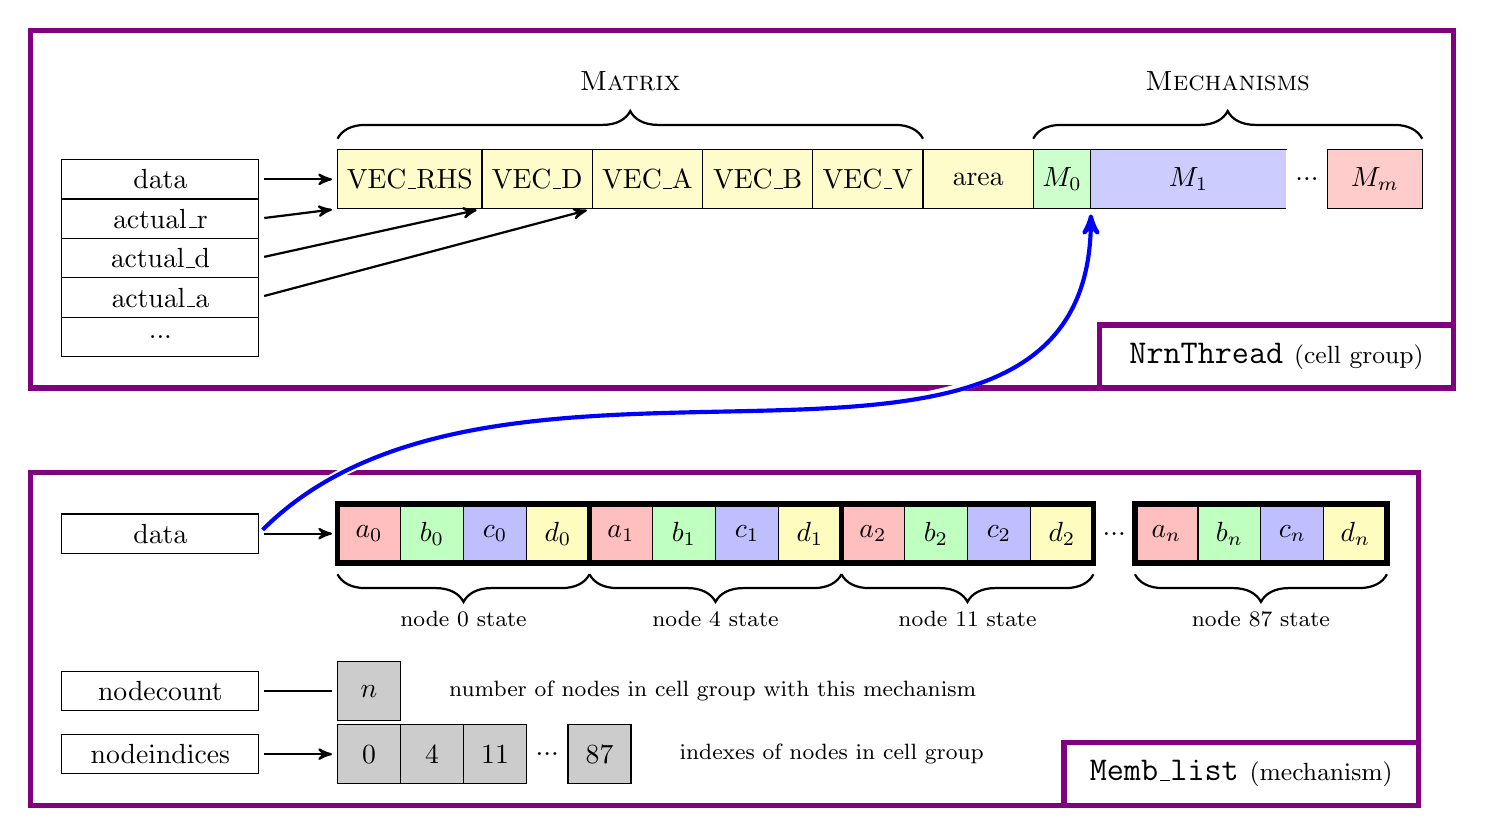
\begin{tikzpicture}[x=0cm, y=0cm, node distance=0 cm,outer sep = 0pt]
\tikzstyle{nvec}=[draw, rectangle,
                  minimum height=\nodeheight, minimum width=\nodewidth,
                  fill=yellow!20,anchor=south west,minimum width=1.4cm]
\tikzstyle{mch0}=[draw, rectangle,
                  minimum height=\nodeheight,
                  fill=green!20,anchor=south west,minimum width=0.5cm]
\tikzstyle{mch1}=[draw, rectangle,
                  minimum height=\nodeheight,
                  fill=blue!20,anchor=south west,minimum width=2.48cm]
\tikzstyle{mch2}=[draw, rectangle,
                  minimum height=\nodeheight,
                  fill=red!20,anchor=south west,minimum width=1.2cm]
\tikzstyle{blank}=[draw=none, rectangle,
                   fill=white, minimum height=\nodeheight,
                   minimum width=0.1cm, anchor=south west]
\tikzstyle{pointer}=[draw=black, fill=white, rectangle,
                   minimum height=0.5cm, minimum width=2.5cm, anchor=south west]

\tikzstyle{t0}=[draw, rectangle,  minimum height=\nodeheight, minimum width=\mechnodewidth,
                fill=red!25,anchor=south west]
\tikzstyle{t1}=[draw, rectangle,  minimum height=\nodeheight, minimum width=\mechnodewidth,
                fill=green!25,anchor=south west]
\tikzstyle{t2}=[draw, rectangle,  minimum height=\nodeheight, minimum width=\mechnodewidth,
                fill=blue!25,anchor=south west]
\tikzstyle{t3}=[draw, rectangle,  minimum height=\nodeheight, minimum width=\mechnodewidth,
                fill=yellow!25,anchor=south west]
\tikzstyle{cover}=[draw, rectangle,  minimum height=\nodeheight, minimum width=3.2cm,
                line width = 2pt,anchor=south west]
\tikzstyle{index}=[draw, rectangle,  minimum height=\nodeheight, minimum width=\mechnodewidth,
                   fill=black!20,anchor=south west]
%%%%%%%%%%%%%%%%%%%%%%%%%%%%%%%%%
% NrnThread
%%%%%%%%%%%%%%%%%%%%%%%%%%%%%%%%%
\node[pointer] (data) at (0,0)         {\lst{data}};
\node[nvec] (vecr)    [right = 1cm of data] {\lst{VEC_RHS}};

\node[nvec] (vecd)    [right = of vecr] {\lst{VEC_D}};
\node[nvec] (veca)    [right = of vecd] {\lst{VEC_A}};
\node[nvec] (vecb)    [right = of veca] {\lst{VEC_B}};
\node[nvec] (vecv)    [right = of vecb] {\lst{VEC_V}};
\node[nvec] (vecarea) [right = of vecv] {\lst{area}};
\node[mch0] (m0)      [right = of vecarea] {$M_0$};
\node[mch1] (m1)      [right = of m0] {$M_1$};
\node[blank](dd)      [right = of m1] {...};
\node[mch2] (m2)      [right = of dd] {$M_{m}$};

\node[pointer] (vecrp)[below = of data] {\lst{actual_r}};
\node[pointer] (vecdp)[below = of vecrp] {\lst{actual_d}};
\node[pointer] (vecap)[below = of vecdp] {\lst{actual_a}};
\node[pointer] (vecetc)[below = of vecap] {\lst{...}};

\path[pil,->] (data.east)  edge (vecr.west);
\path[pil,->] (vecrp.east) edge (vecr.south west);
\path[pil,->] (vecdp.east) edge (vecd.south west);
\path[pil,->] (vecap.east) edge (veca.south west);


\draw[decorate,decoration={brace,raise=4pt,amplitude=10pt},thick]
  (vecr.north west)--(vecv.north east)
  node[midway,yshift=25pt] (matbrace) {\sc Matrix};

\draw[decorate,decoration={brace,raise=4pt,amplitude=10pt},thick]
  (m0.north west)--(m2.north east)
  node[midway,yshift=25pt] (mechbrace) {\sc Mechanisms};

\tikzset{typeline/.style={draw=blue!50!red, line width=2pt,
                          inner sep=4mm, rectangle}};
\node (nrnthread)[typeline,
                  fit = (vecr)(data)(vecd)(veca)(vecb)(vecv)(vecarea)
                        (m0)(m1)(dd)(m2)
                        (matbrace)(mechbrace)
                        (vecrp)(vecap)(vecdp)(vecetc)] {};

\node at (nrnthread.south east)
    [anchor=south east, fill=white, draw=red!50!blue, line width=2pt, minimum height=0.8cm, minimum width=4.5cm]
    {\large {\texttt{NrnThread}} \small (cell group)};

%%%%%%%%%%%%%%%%%%%%%%%%%%%%%%%%%
% Memb_list
%%%%%%%%%%%%%%%%%%%%%%%%%%%%%%%%%

\node[pointer] (datamech)[below = 2cm of vecetc] {\lst{data}};
\node[t0] (m00) [right = 1cm of datamech] {$a_0$};
\node[t1] (m01) [right = of m00] {$b_0$};
\node[t2] (m02) [right = of m01] {$c_0$};
\node[t3] (m03) [right = of m02] {$d_0$};
\node[t0] (m10) [right = of m03] {$a_1$};
\node[t1] (m11) [right = of m10] {$b_1$};
\node[t2] (m12) [right = of m11] {$c_1$};
\node[t3] (m13) [right = of m12] {$d_1$};
\node[t0] (m20) [right = of m13] {$a_2$};
\node[t1] (m21) [right = of m20] {$b_2$};
\node[t2] (m22) [right = of m21] {$c_2$};
\node[t3] (m23) [right = of m22] {$d_2$};
\node[blank] (blank) [right = of m23] {...};
\node[t0] (m30) [right = of blank] {${a_n}$};
\node[t1] (m31) [right = of m30] {${b_n}$};
\node[t2] (m32) [right = of m31] {${c_n}$};\\
\node[t3] (m33) [right = of m32] {${d_n}$};\\

\node[cover] (n1)[left = of m10] {};
\node[cover] (n2)[left = of m20] {};
\node[cover] (n3)[left = of blank] {};
\node[cover] (n4)[right = of blank] {};

\path[pil,->] (datamech.east) edge (m00.west);

\node[pointer] (nodecount)[below = 1.5cm of datamech] {\lst{nodecount}};
\node[pointer] (nodeindices)[below = 0.3cm of nodecount] {\lst{nodeindices}};

\node[index] (nc) [right = 1cm of nodecount] {$n$};
\node (nclabel)[right = 0.5cm of nc] {\footnotesize number of nodes in cell group with this mechanism};
\node[index] (ni1)[right = 1cm of nodeindices] {0};
\node[index] (ni2)[right = of ni1] {4};
\node[index] (ni3)[right = of ni2] {11};
\node[blank] (blankni)[right = of ni3] {...};
\node[index] (ni4)[right = of blankni] {87};
\node (nilabel)[right = 0.5cm of ni4] {\footnotesize indexes of nodes in cell group};
\path[pil,->] (nodeindices.east) edge (ni1.west);
\path[pil,-]  (nodecount.east) edge (nc.west);

%\path[pil,-] (ni4.east) edge (nilabel.west);
%\path[pil,-] (nc.east) edge  [draw=blue, line width=1pt] (nclabel.west);


\draw[decorate,decoration={brace,raise=4pt,mirror,amplitude=10pt},thick]
  (n1.south west)--(n1.south east)
  node[midway,yshift=-20pt] (node0) {\footnotesize node 0 state};
\draw[decorate,decoration={brace,raise=4pt,mirror,amplitude=10pt},thick]
  (n2.south west)--(n2.south east)
  node[midway,yshift=-20pt] (node1) {\footnotesize node 4 state};
\draw[decorate,decoration={brace,raise=4pt,mirror,amplitude=10pt},thick]
  (n3.south west)--(n3.south east)
  node[midway,yshift=-20pt] (node2) {\footnotesize node 11 state};
\draw[decorate,decoration={brace,raise=4pt,mirror,amplitude=10pt},thick]
  (n4.south west)--(n4.south east)
  node[midway,yshift=-20pt] (node3) {\footnotesize node 87 state};

\node (memblist)[typeline,
                  fit = (datamech)(m33)(node3)(nodeindices)] {};

\node at (memblist.south east)
    [anchor=south east, fill=white, draw=red!50!blue, line width=2pt, minimum height=0.8cm, minimum width=4.5cm]
    {\large {\texttt{Memb\_list}} \small (mechanism)};

\path[pil,-] (datamech.east) edge  [out=45, in=-90, draw=white, line width=3pt] (m1.south west);
\path[pil,->] (datamech.east) edge  [out=45, in=-90, draw=blue, line width=1.5pt] (m1.south west);


\end{tikzpicture}
\end{document}

